\begingroup
\widowpenalty=10000
\clubpenalty=10000
\section{Mở rộng dữ liệu phụ trợ và năng lực suy luận}
\label{sec:expanded-shadow-experiment}

\subsection{Câu hỏi kiểm tra và giả định đối thủ}

Phép kiểm tra giữ nguyên bảy cơ chế, $K=5$, ngân sách $0{,}24/\mathrm m$, đầu ra và utility của vòng phân rã prior. Thành phần thay đổi là đối thủ: liệu kết quả riêng tư còn giữ khi đối thủ có dữ liệu phụ trợ rộng hơn và phép suy luận phi tuyến? Cấu hình bảo vệ $U/U$ đã chọn không được chọn lại; bốn nhóm 201--204 vẫn là dữ liệu phát triển đã xem, không trở thành xác nhận mới.

Đối thủ biết cơ chế và bản đồ, có thể chạy cơ chế trên tuyến mô phỏng để tạo cặp đầu ra công khai--vị trí thật cho học. Nguồn phụ trợ tổng hợp là giả định cần xét: Guan và cộng sự sử dụng tuyến tổng hợp cho suy luận thành viên trên dữ liệu vị trí tổng hợp.~\citep{guan2024synthetic} Tuy nhiên mục tiêu và đầu ra của họ khác bài toán ở đây; thí nghiệm này suy luận tọa độ từ chuỗi dummy, không tái hiện tấn công đó và không giả định đối thủ hoàn toàn không có dữ liệu phụ trợ.

\subsection{Bộ học và các quyết định bổ sung}

Bộ dữ liệu ở Mục~\ref{sec:auxiliary-shadow-data} bổ sung 64 nhóm học và giữ lại 16 nhóm riêng. Mỗi cấu hình tạo đầu ra cho 256 cửa sổ học, với một lần sinh ngẫu nhiên trên mỗi cửa sổ; các cấu hình dùng neo ngẫu nhiên ghép cặp. Ghép với 360 quan sát cũ, mỗi bộ học có 3.233 quan sát và 1.381 tọa độ khác nhau từ 66 nhóm tuyến. Các cửa sổ dừng/quay lại cùng nhóm có liên quan; đây là học theo trọng số quan sát, không phải lấy mẫu người dùng độc lập hay phân bố cư dân đã hiệu chuẩn.

\begin{figure}[htbp]
\centering
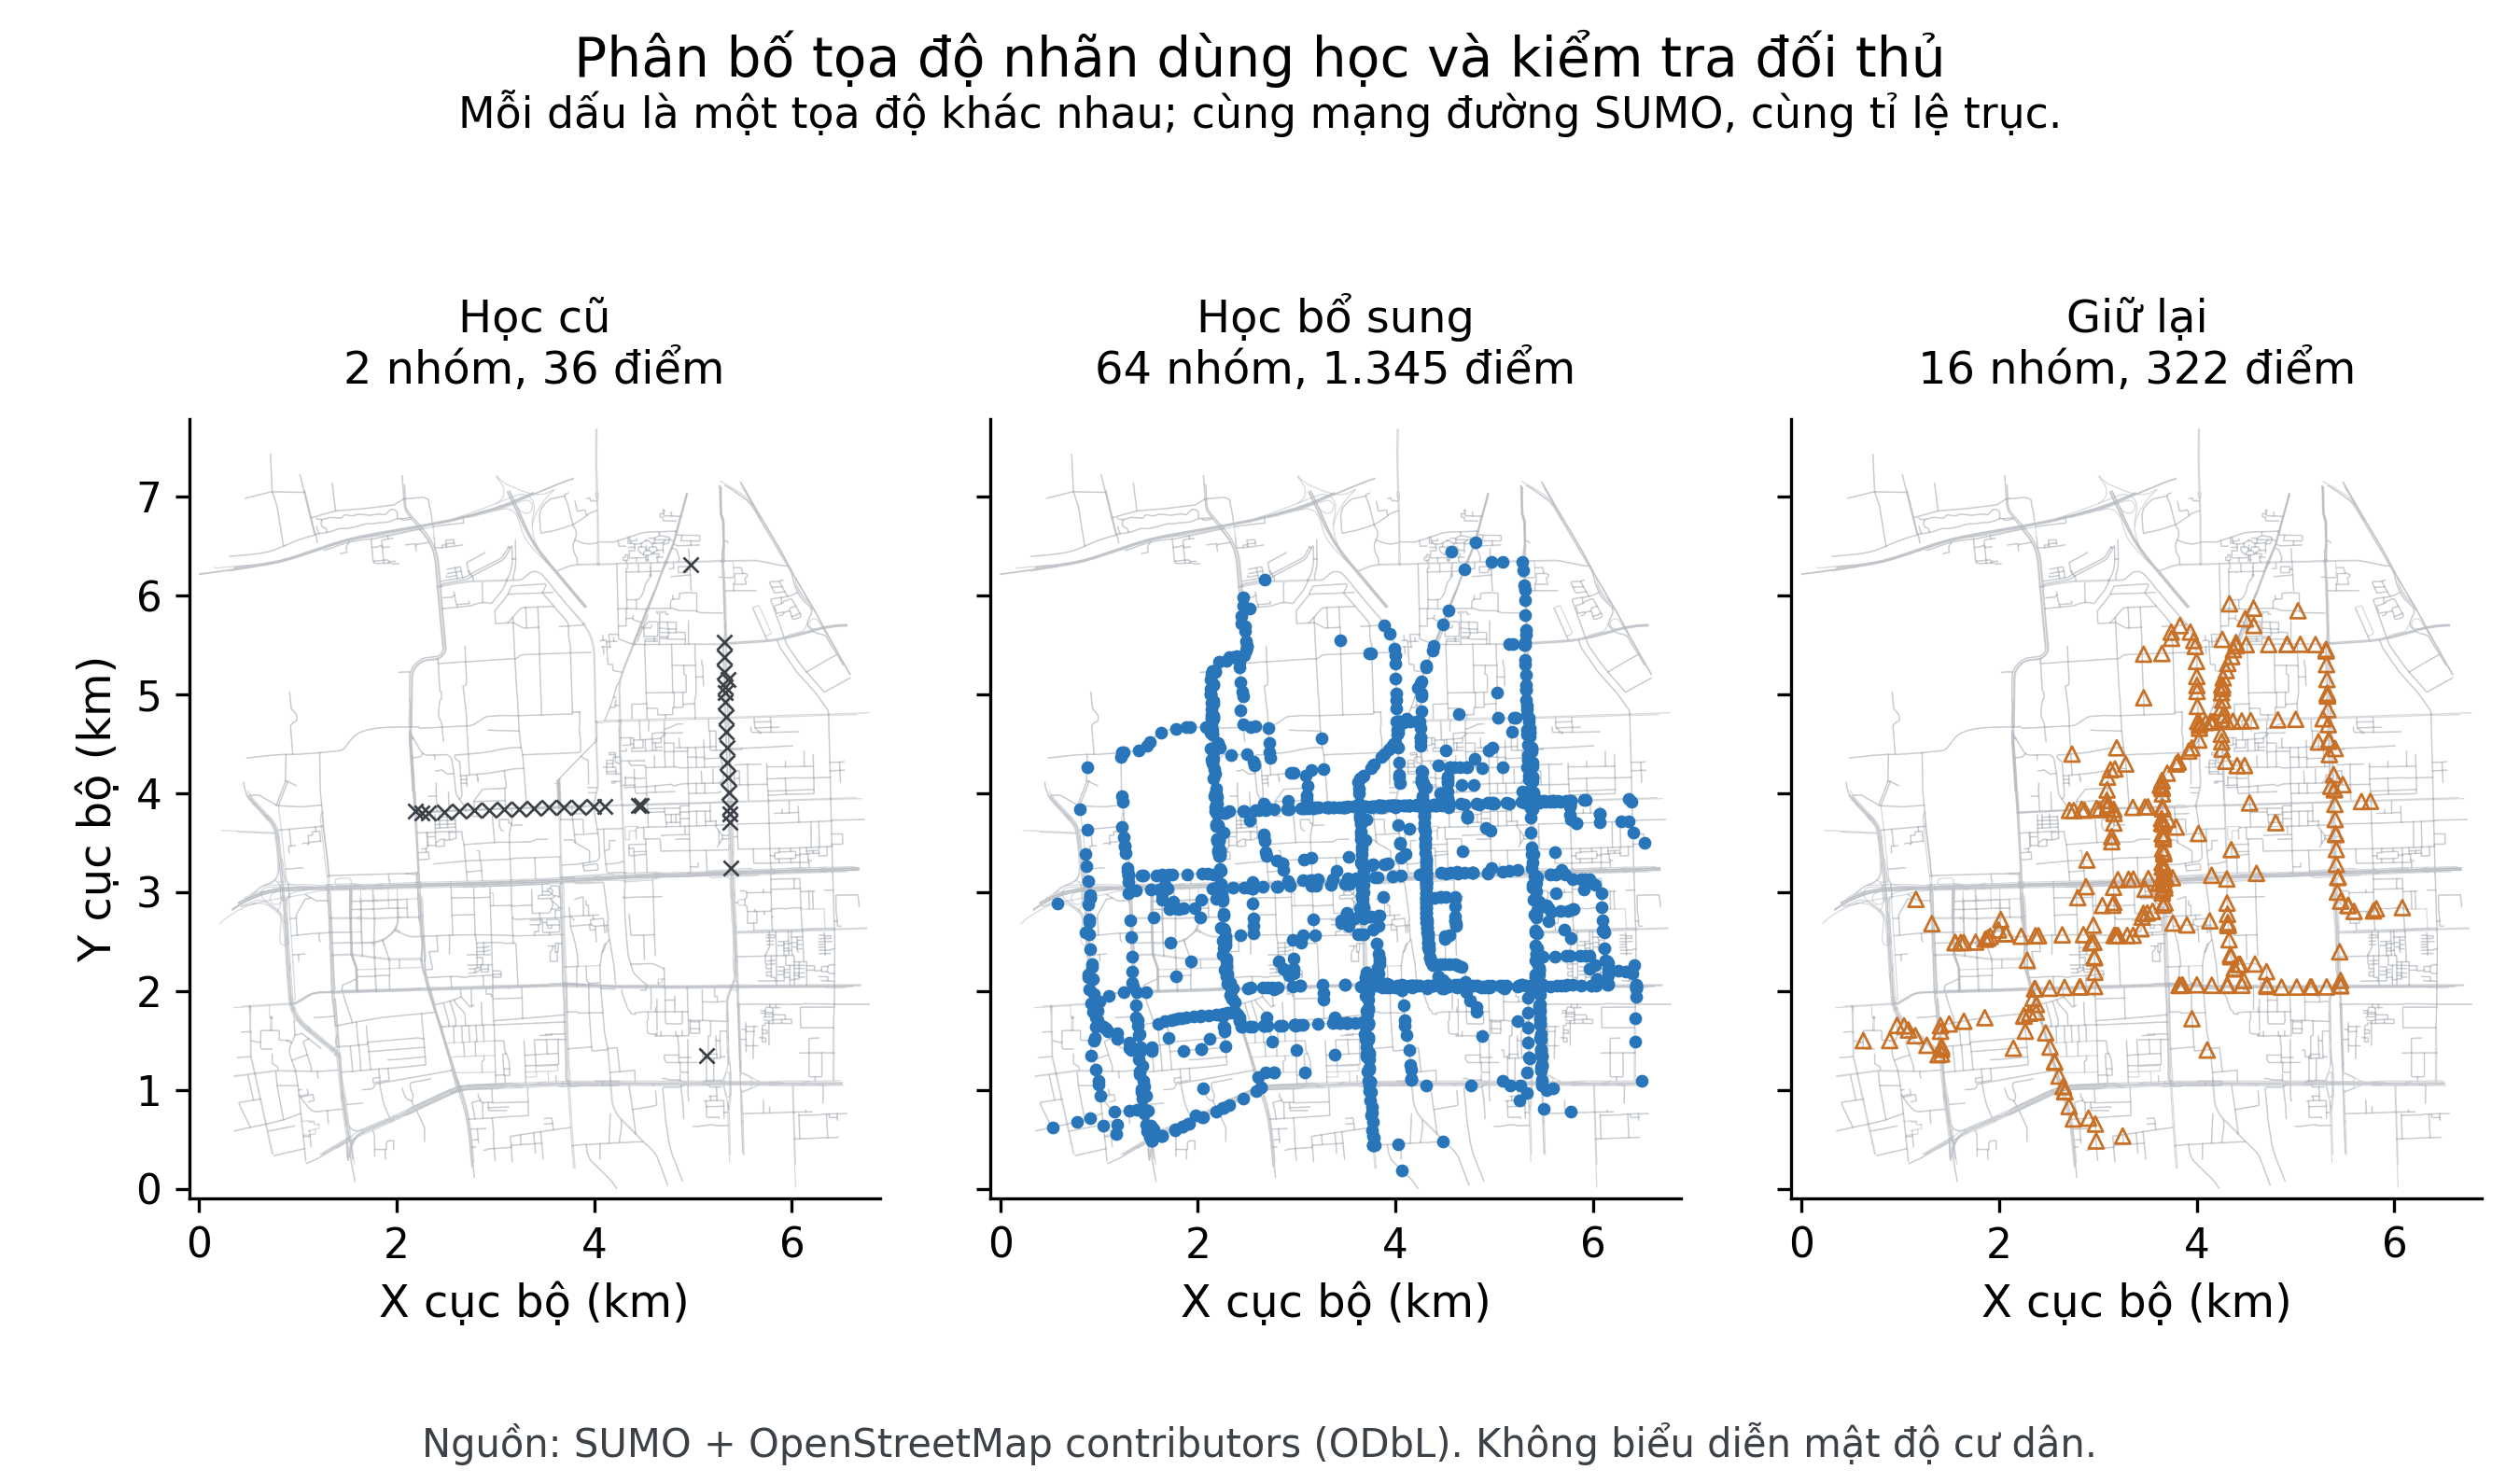
\includegraphics[width=\textwidth]{../artifacts/datasets/urban_shadow_v1/spatial_support.png}
\caption{Độ phủ tọa độ nhãn trước và sau mở rộng. Mọi điểm GPS được đổi về cùng hệ tọa độ SUMO; mỗi dấu là một tọa độ khác nhau. Tập giữ lại có thể đi trên đường chung với tập học.}
\label{fig:expanded-shadow-support}
\end{figure}

Mỗi sự kiện được biểu diễn bằng 21 đặc trưng công khai: mười thành phần tọa độ của năm dummy theo thứ tự cố định, mười thành phần trung bình tiền tố và thời gian đã trôi qua. Chuẩn hóa chỉ dùng tập học. Vị trí thật, neo riêng tư, làn thật, tốc độ thật, nhãn kịch bản và phần tương lai không đi vào mô hình suy luận. Đối thủ cũ quan sát cả cửa sổ vẫn được giữ; chỉ các mô hình học mới bị giới hạn ở đặc trưng tiền tố.

Thêm tám quyết định cùng dạng với vòng trước nhưng học lại trên dữ liệu rộng hơn: trung bình 1/5/15 láng giềng, quyết định MAE và Hit với 15/45 láng giềng, cùng trung bình 45 láng giềng. Đối chiếu này tách tác động tăng dữ liệu khỏi thay kiến trúc học. Thêm hai bộ hồi quy ExtraTrees: dự đoán trực tiếp tọa độ và dự đoán phần lệch so với tâm năm dummy hiện tại rồi cộng tâm trở lại. Mỗi bộ có 128 cây, độ sâu tối đa 18, ít nhất năm mẫu ở lá; một đặc trưng được lấy ngẫu nhiên tại mỗi lần tách nút. Tham số và seed được cố định trước khi chấm, không tìm lại theo kết quả.

Hai bộ cây tối ưu sai số bình phương, không phải trực tiếp MAE hoặc Hit. Các quyết định láng giềng tối ưu mất mát trên một phân bố thực nghiệm hữu hạn, chưa phải hậu nghiệm đúng cơ chế.~\citep{shokri2015privacygames} Điểm đoán được phép nằm ngoài đường hoặc tập dummy và được chấm với GPS thật. Dung sai trong dựng hình học không được cộng vào ngưỡng Hit: phép chấm vẫn dùng khoảng cách $\leq100$ m.

\subsection{Chọn đối thủ và kiểm tra chuyển giao}

Nhóm 103/104 chọn một đối thủ cho từng cấu hình, ca và phép đo; không dùng nhãn phát triển để chọn. Giữ cả lựa chọn cũ và lựa chọn mở rộng. Bao đối thủ thăm dò lấy cực đại Hit hoặc cực tiểu MAE trong từng ca trên tập phát triển rồi mới trung bình, không phải kết quả xác nhận của một đối thủ đã khóa. Vì giữ toàn bộ bộ cũ, bao Hit mới không thể giảm và bao MAE mới không thể tăng; đây là tính chất bao hàm tập đối thủ, không là bảo đảm rằng lựa chọn validation luôn tốt hơn.

Để chấm 16 nhóm phụ trợ giữ lại, chọn một đối thủ toàn cục cho mỗi cấu hình và phép đo bằng trung bình chín ca validation cũ, chỉ xét đối thủ có mặt ở mọi ca. Không chọn lại riêng theo bốn dạng cửa sổ giữ lại. Dữ liệu này có tuyến chưa dùng để học nhưng vẫn chung bản đồ và không được sinh từ điều kiện hợp lệ của chín ca chính; kết quả chỉ đánh giá chuyển giao sang lịch quan sát phụ trợ.

\begin{table}[htbp]
\centering\small
\caption{Suy luận trên cùng đầu ra của bốn nhóm phát triển 201--204; chín ca, $K=5$. Đối thủ chọn trên 103/104 riêng cho từng ca và phép đo. Hit tính bằng \%, MAE bằng m.}
\label{tab:expanded-shadow-selected}
\begin{tabular}{lrrrr}
\toprule
Cấu hình & Hit chọn cũ & Hit chọn mới & MAE chọn cũ & MAE chọn mới\\
\midrule
BR-làn & 8.46 & 8.65 & 744.8 & 747.9 \\
L/L & 0.00 & 3.86 & 1467.2 & 1173.4 \\
U/U & 2.78 & 3.76 & 1283.6 & 1110.1 \\
L/U & 0.00 & 3.86 & 1449.3 & 1165.7 \\
U/L & 2.78 & 5.47 & 1316.5 & 1165.5 \\
C/C & 1.00 & 2.08 & 1263.4 & 962.0 \\
M/M & 2.08 & 1.47 & 1082.9 & 1082.9 \\
\bottomrule
\end{tabular}
\end{table}
\begin{table}[htbp]
\centering\small
\caption{Bao đối thủ thăm dò trên cùng tập phát triển: cực đại Hit (\%) và cực tiểu MAE (m) trong từng ca, rồi lấy trung bình chín ca. Đây không phải điểm xác nhận của đối thủ đã chọn.}
\label{tab:expanded-shadow-envelope}
\begin{tabular}{lrrrr}
\toprule
Cấu hình & Hit bao cũ & Hit bao mới & MAE bao cũ & MAE bao mới\\
\midrule
BR-làn & 16.81 & 17.05 & 429.5 & 426.1 \\
L/L & 5.06 & 9.59 & 1188.9 & 782.9 \\
U/U & 14.30 & 16.23 & 508.2 & 503.8 \\
L/U & 5.20 & 8.98 & 1179.2 & 787.0 \\
U/L & 14.14 & 16.15 & 519.9 & 513.0 \\
C/C & 6.42 & 9.20 & 1152.2 & 753.1 \\
M/M & 8.72 & 9.93 & 539.0 & 526.3 \\
\bottomrule
\end{tabular}
\end{table}
\begin{table}[htbp]
\centering\small
\caption{Chuyển giao đối thủ sang 16 nhóm phụ trợ giữ lại, cấu hình $U/U$. Một đối thủ toàn cục cho mỗi phép đo được chọn trên chín ca validation cũ, không chọn lại theo cửa sổ giữ lại.}
\label{tab:expanded-shadow-holdout}
\begin{tabular}{lrrrr}
\toprule
Cửa sổ & Hit cũ (\%) & Hit mới (\%) & MAE cũ (m) & MAE mới (m)\\
\midrule
Di chuyển 20 s & 4.17 & 2.60 & 1391.9 & 1391.9 \\
Di chuyển 60 s & 2.85 & 3.14 & 1472.7 & 1472.7 \\
Quay lại 5 s & 9.38 & 3.12 & 1377.2 & 1377.2 \\
Dừng 5 s & 0.00 & 0.00 & 1485.6 & 1485.6 \\
\bottomrule
\end{tabular}
\end{table}
\begin{table}[htbp]
\centering\small
\caption{Tách ảnh hưởng mở rộng bộ học ở $U/U$: từng đối thủ cố định trên chín ca phát triển. Các hàng này là phân tích thành phần, không thay điểm của đối thủ đã chọn bằng validation.}
\label{tab:expanded-shadow-data-effect}
\begin{tabular}{lrrrr}
\toprule
Đối thủ & MAE cũ (m) & MAE mới (m) & Hit cũ (\%) & Hit mới (\%)\\
\midrule
1-NN & 1486.7 & 802.6 & 2.78 & 4.50 \\
Trung bình 5 & 1449.5 & 777.4 & 0.42 & 2.72 \\
Trung bình 15 & 1749.0 & 775.7 & 0.31 & 0.89 \\
MAE, 15 nhãn & 2048.4 & 832.6 & 0.15 & 3.02 \\
Hit, 15 nhãn & 1941.5 & 837.2 & 2.78 & 4.56 \\
MAE, 45 nhãn & 2188.5 & 730.1 & 0.00 & 4.08 \\
Hit, 45 nhãn & 2384.1 & 886.8 & 0.00 & 2.33 \\
Trung bình 45 & 1917.2 & 683.5 & 0.00 & 1.49 \\
Cây: tọa độ & --- & 660.2 & --- & 1.34 \\
Cây: phần lệch & --- & 550.4 & --- & 3.41 \\
\bottomrule
\end{tabular}
\end{table}


Trên cùng đầu ra $U/U$, Hit của đối thủ chọn bằng validation tăng từ 2,78\% lên 3,76\%, còn MAE giảm từ 1.283,6 m xuống 1.110,1 m. Bao Hit thăm dò tăng từ 14,30\% lên 16,23\%. Cả hai thay đổi cho thấy các phép đo cũ chưa khai thác hết rò rỉ có thể suy luận bằng bộ mới; chúng không thể hiện cải tiến cơ chế bảo vệ. Recall $U/U$ vẫn là 92,35\%, ca thấp nhất 86,01\%, nên ràng buộc utility từng ca chưa đạt.

Tuy nhiên, bao MAE thăm dò của $U/U$ chỉ giảm từ 508,2 m xuống 503,8 m. Vì bộ cũ đã có đối thủ đạt sai số thấp ở từng ca, mức giảm lớn hơn của MAE chọn không đồng nghĩa với tăng mạnh năng lực tốt nhất trong toàn bộ bộ đối thủ. Phải xét cả hai bảng để tránh phóng đại tác động mở rộng dữ liệu.

Kết quả không tăng đồng đều theo mọi lựa chọn. Với $M/M$, Hit của đối thủ được chọn giảm từ 2,08\% xuống 1,47\%, trong khi bao Hit thăm dò tăng từ 8,72\% lên 9,93\%. Đây là phản ví dụ về khả năng chuyển giao lựa chọn từ hai nhóm validation: thêm đối thủ có thể làm lộ thêm điểm yếu nhưng vẫn chọn nhầm đối thủ cho nhóm khác. Không được dùng mức Hit chọn thấp hơn để tuyên bố $M/M$ riêng tư hơn trong vòng kiểm tra này.

Phân tích từng quy tắc cố định ở Bảng~\ref{tab:expanded-shadow-data-effect} làm rõ tác động dữ liệu. Ở $U/U$, cùng quy tắc 1-NN giảm MAE từ 1.486,7 m xuống 802,6 m khi mở rộng bộ học. Bộ cây dự đoán phần lệch đạt 550,4 m trên trung bình chín ca phát triển, nhưng không được chọn làm đối thủ MAE toàn cục trên validation. Khoảng cách này cho thấy tăng năng lực bộ đối thủ và chọn được đối thủ chuyển giao tốt là hai yêu cầu khác nhau. Không lấy điểm phát triển thuận lợi để sửa lại lựa chọn đã khóa.

Tập phụ trợ giữ lại cung cấp thêm phản ví dụ. Với $U/U$, Hit của đối thủ toàn cục mới giảm từ 4,17\% xuống 2,60\% ở cửa sổ di chuyển 20 giây và từ 9,38\% xuống 3,12\% ở cửa sổ quay lại; ở cửa sổ 60 giây tăng từ 2,85\% lên 3,14\%. Lựa chọn MAE toàn cục vẫn là đối thủ 1-NN cũ nên MAE giữ nguyên. Như vậy, mở rộng dữ liệu học đã tăng khả năng của một số phép suy luận, nhưng bộ chọn từ hai nhóm validation chưa chuyển giao ổn định sang lịch quan sát khác.

\subsection{Điều kiện để kết luận về riêng tư}

Đánh giá lại cùng đầu ra giúp quy thay đổi điểm suy luận cho bộ đối thủ, không nhầm với cải tiến cơ chế bảo vệ. Ngược lại, nếu điểm của một đối thủ mới kém hơn, đó có thể là lệch phân bố, thiếu đặc trưng hoặc quá khớp tập chọn nhỏ; không phải bằng chứng người dùng được bảo vệ tốt hơn. Kiểm tra tiếp theo cần nhiều nhóm chọn độc lập, đặc trưng chuyển động/ngữ nghĩa mạnh hơn hoặc likelihood đúng cơ chế, và tập xác nhận mới sau khi khóa phương pháp. Các kết quả hữu hạn không chặn năng lực mọi đối thủ, không chứng minh mới về Geo-I và chưa mở rộng bảo vệ đo được sang S4--S8.
\par\endgroup
